\documentclass[11pt, oneside]{article}   	% use "amsart" instead of "article" for AMSLaTeX format
\usepackage{geometry}                		% See geometry.pdf to learn the layout options. There are lots.
\geometry{letterpaper}                   		% ... or a4paper or a5paper or ... 

\usepackage[english]{babel}
\usepackage{url}
\usepackage{pstricks, tikz}
\usepackage[T1]{fontenc}
\usepackage{setspace}
\usepackage{graphicx}
\usepackage[normalem]{ulem} %for \sout
\usepackage{amssymb}
\usepackage{color}
\usepackage{tipa}
\usepackage{multicol}
\usepackage{linguex} %declare this package after tipa and graphicx
\renewcommand{\firstrefdash}{}
\usepackage{qtree}
\usepackage{tree-dvips} %copy tree-dvips folder to make this work
\qtreecenterfalse

\usepackage{fancyhdr}
\pagestyle{fancy}{
\fancyhead[L]{Roberto Petrosino}
\fancyhead[C]{LING2010Q}
\fancyhead[R]{1: Intro to linguistics}
\renewcommand{\footrulewidth}{0pt}
\renewcommand{\headrulewidth}{0pt}}

\newenvironment{packed_enum}{
\begin{enumerate}
  \setlength{\itemsep}{1pt}
  \setlength{\parskip}{0pt}
  \setlength{\parsep}{0pt}
}{\end{enumerate}}

\newenvironment{packed_item}{
\begin{itemize}
  \setlength{\itemsep}{1pt}
  \setlength{\parskip}{0pt}
  \setlength{\parsep}{0pt}
}{\end{itemize}}

\renewcommand{\labelitemiii}{$\diamond$}


\title{{\normalsize LING 2010Q -- {\scshape Fall 2017}} \\ {\bfseries 1 - Intro to Linguistics}, or: \\ {\itshape what exactly do you linguists do for a living?}}
\author{Roberto Petrosino \\ \url{roberto.petrosino@uconn.edu}}
\date{\today}

\begin{document}

\maketitle
\tableofcontents

\newpage

\section{Is language innate?}

\ex. {\bfseries Behavioralists} believe that language acquisition results from direct association between {\itshape stimulus} and {\itshape response} (Skinner 1957). As a consequence, acquiring a language means memorizing all possible sentences in a given language. \underline{However}:
\a. Our memory capacities would need to be powerful enough to do that ? and we are yet far from understanding it wholly.
\b. On top of that, consider the following sentences and complete accordingly, by using your intuition:
	\a. The man is tall.  			\hfill	$\rightarrow$  \hspace{0.2cm} 	Is the man tall?
	\b. The man kisses the girl. 	\hfill	$\rightarrow$  \hspace{0.2cm}	\underline{\hspace{2.65cm}}
	\c. The man kissed the girl 	\hfill	$\rightarrow$  \hspace{0.2cm}	\underline{\hspace{2.65cm}}	
	\d. The man has kissed the girl.  \hfill	$\rightarrow$  \hspace{0.2cm}	\underline{\hspace{2.65cm}}
	\e. The man who runs has kissed the girl. 	\hfill	$\rightarrow$  \hspace{0.2cm}	\underline{\hspace{2.65cm}}

What I am getting at? Assuming that language acquisition occurs through memorization is obviously wrong - what would (a-e) have been, if that assumption was correct? \\

{\itshape Your answer}:

\vspace{1.5cm}

\ex. {\bfseries Generativists} believe that language must have (some degree of) innateness: we are factually born with specific abilities, which make us able to acquire our native language when we were kids. This occurs:
\a. {\itshape effortlessly} --- children typically manage to master their native language by the age of 5. Strikingly, when they speak, they make very few errors.
\b. in spite of the so-called poverty of stimulus: children just pick a language, although the input is typically:
	\a. {\itshape noisy} --- when we speak, we provide with a signal full of errors, interruptions, breaks
	\b. {\itshape limited} --- if we reckon the great amount of possibilities to mean the same thing with different words; on top of that, children do not seem to rely on {\itshape negative evidence} (i.e., direct teaching of what is grammatically wrong) at all.

\ex. The bullets above are also known as the {\bfseries logic problem of language acquisition}, already recognized by Plato (V-IV BC). 

\ex. The immediate consequence is that we must be endowed with a {\bfseries {\itshape somewhat innate} faculty of language}, which allows children to manipulate the stimulus and acquire a language from it.

\subsection{A trio of abilities}

\ex. {\bfseries Displaced reference}, the ability of talking about something afar from `here and now'. 

\begin{quote}
For example, I can tell you about my family in Italy (3,600+ miles away: {\itshape spatial distance}) or about my recent vacation in Germany (a couple of weeks ago: {\itshape temporal distance}); if I were an astronaut traveling the cosmos, I could have talked about my last trip to Kepler-186f (490 light years: {\itshape spatio-temporal distance}).
\end{quote}

\ex. {\bfseries Discreteness}, the ability of using a fixed inventory of `building blocks' which can be combined to form bigger units. 

\begin{center}
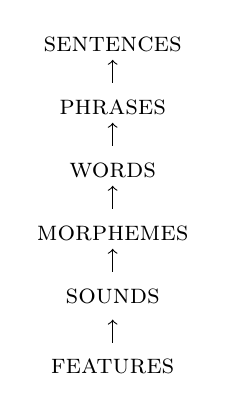
\begin{tikzpicture}

	\node[align=center] at (0, 3.5) {\scshape sentences};
		\draw[<-] (0, 3.3) -- (0, 3);
	\node[align=center] at (0, 2.7) {\scshape phrases};
		\draw[<-] (0, 2.5) -- (0, 2.2);
	\node[align=center] at (0, 1.9) {\scshape words};
		\draw[<-] (0, 1.7) -- (0, 1.4);
	\node[align=center] at (0, 1.1) {\scshape morphemes};
		\draw[<-] (0, 0.9) -- (0, 0.6);
	\node[align=center] at (0, 0.3) {\scshape sounds};
		\draw[<-] (0, 0) -- (0, -0.3);
	\node[align=center] at (0, -0.6) {\scshape features};
	
\end{tikzpicture}
\end{center}

\ex. {\bfseries Recursion}, the ability of applying whatever operation over and over: 
\a. {[John is sad]}
\b. {[Dorothy thinks that [John is sad]]}
\c. {[Toto suspects that [Dorothy thinks that [John is sad]]]}
\d. {[Lucy wonders whether [Toto suspects that [Dorothy thinks that [John is sad]]]]} \\
\e.[] \hfill {\itshape ...and so on}

\section{Grammars}

\subsection{Generative grammar}

\ex. {\bfseries Open-endedness}. We are able to make use a limited set of linguistic rules to mean the same thing in a potentially infinite number of ways.

\ex. {\bfseries Creativity}. Speakers can therefore produce and understand any number of messages that have {\itshape never been expressed before}, also thanks to recursion.
\a. Colorless green ideas sleep furiously. (Chomsky, 1957)
\b. Pink elephants were dancing on TV when the astronaut called home to say that he got safely to Mars. (Roberto, 2017)
\c. I'm so hungry that I could {\itshape devour} you in one bite! (Sophia, $\sim$3 yy.o.o., 2009)

\ex. {\bfseries Tacit knowledge}. We all know how to speak our native languages without being taught --- we {\itshape just }know it. 

\subsubsection{Activity 1: Systematic and accidental gaps}

{\itshape Look at the following pseudo-words; following your intuition, which of them are possible words in English? Check the corresponding box.}

\parbox{.5\textwidth}{%
   \begin{enumerate}
    \item mbood\hfill \framebox(10,10){}
    \item frall\hfill \framebox(10,10){}
    \item coofp\hfill \framebox(10,10){}
    \item ktleem\hfill \framebox(10,10){}
    \item flube \hfill \framebox(10,10){}
    \item sglop \hfill \framebox(10,10){}
    \item blick \hfill \framebox(10,10){}
    \item bnick \hfill \framebox(10,10){}
    \item strick\hfill \framebox(10,10){}
    \end{enumerate}%
}

\ex. Halle (1973):
\a. Unchecked words are examples of {\itshape systematic gaps} --- they do not exist in a language due to language-specific constraints (at the phonological, morphological, syntactic or semantic level).
\b. Checked words are {\itshape accidental gaps} --- they do not exist in some language, but which would be permitted by the grammatical rules of the language. 

\subsubsection{Activity 2: {\itshape Wanna}-contraction}

{\itshape Consider the following sentence:}

\ex. Nathan Petrelli is a politician I want to succeed.

\newpage

This sentence has two meanings - describe them:

\begin{enumerate}
	\item 
	\item	
\end{enumerate}
 
 \noindent {\itshape By comparison, consider sentence \Next. What does it mean?}
 
\ex. Nathan Petrelli is a politician I wanna succeed.
 
\par {\itshape Your answer:}
 
\vspace{1.5cm} 


\noindent {\itshape Now consider some more sentence pairs similar to \LLast and \Last:}

\ex. \label{1} \a. The student who cheated on the exam is the one I want to fail.
\b.The student who cheated on the exam is the one I wanna fail.

\ex. \label{2} \a. Fedora Saura is a racehorse I want to win.
\b. Fedora Saura is a racehorse I wanna win.

\ex. \label{3} \a. The Braeburn is a variety of apple I want to grow here.
\b. The Braeburn is a variety of apple I wanna grow here.

{\itshape Do the sentences in \ref{1}a, \ref{2}a, \ref{3}a have one possible meaning, or two? \\

Your answer:} \\

\vspace{1.5cm}


\noindent {\itshape Do the sentences in \ref{1}b, \ref{2}b, \ref{3}b have one possible meaning, or two? \\

Your answer:} \\

\vspace{1.5cm}

\noindent {\itshape Notice a pattern? If so, were you aware of this before? \\

Your answer:} \\

\vspace{1cm}

\subsubsection{Activity 3: Grammaticality judgments}

{\itshape Which of the following sentences are possible English sentences? Check the corresponding box.}

\parbox{.5\textwidth}{%
   \begin{enumerate}
    \item Colin made Jane a sandwich. \hfill \framebox(10,10){}
    \item John prepared Mary a cake. \hfill \framebox(10,10){}
    \item Cate cleaned the garden up. \hfill \framebox(10,10){}
    \item Cate cleaned up the garden. \hfill \framebox(10,10){}
    \item Cate cleaned up it. \hfill \framebox(10,10){}
    \end{enumerate}%
}

\subsection{Levels of linguistic analysis}

\begin{itemize}
\item {\bf Phonology:} patterns of speech sounds
\begin{itemize}
\item Are the following possible word-beginnings in English? How about word-endings?

\ex. \a. pl
\b. lp
\b. tl%Good in Nahuatl
\b. lt
\c. n
\c. \textipa{N}
\c. \textipa{Z}

\item How many consonants in a row can begin a word in English?
\item Which are natural pronunciations of the word ``ride'' and ``rider''?

\ex. \a. \textipa{\textturnr ajd}
\b. \textipa{\textturnr ajR}
\b. \textipa{\textturnr ajd@\textturnr}
\b. \textipa{\textturnr ajR@\textturnr}

\end{itemize}
\item {\bf Morphology:} patterns within words
\begin{itemize}
\item How many distinct meaningful pieces are inside of the word \textit{underwhelming}?
\item What does the following large compound word mean?

\ex. red wine soaked goat milk cheese

\item Which of the following are possible words in English? (Why or why not?)

\ex. \a. drinkable
\b. openable
\c. chocolateable
\d. prettyable

\ex. \a. dance -- danced
\b. open -- opened
\b. freeze -- freezed
\b. freeze -- froze
\c. squeeze -- squoze

\end{itemize}
\item {\bf Syntax:} patterns within phrases and sentences
\begin{itemize}
\item Which of the following are possible (neutral or non-neutral) sentences of English?

\ex. \a. Julia squashed the bug. %English
\b. The bug squashed Julia. %Hixkaryana
\c. Julia the bug squashed. %Japanese
\d. The bug Julia squashed. %Nadeb
\d. Squashed Julia the bug. %Q'anjob'al
\d. Squashed the bug Julia. %Malagasy

\item In which of the following sentences can ``Carol'' and ``she'' refer to the same person? Why?

\ex. \a. Carol loves her.
\b. Carol thinks that Michael loves her.
\c. Carol thinks that she loves Michael.
\d. She loves Carol.
\d. She thinks that Michael loves Carol.x
\d. She thinks that Carol loves Michael.

\item How does your hypothesis hold up to the following sentences?

\ex. \a. For her final act, Carol juggled five bowling pins.
\b. The terrible picture of her shocked Carol.

\newpage

\item Which of the following sentences are grammatical?

\begin{multicols}{2}{
\ex. \a. I think Craig left.
\b. I think that Craig left.
\c. Who do you think left?
\d. Who you think that left?

}\end{multicols}

\item In the following sentence, which words are most closely related to each other?

\ex. Julia mercilessly squashed the giant blue bug with her foot.

\end{itemize}
\item {\bf Semantics:} meaning computation
\begin{itemize}
\item Are the following sentences true?

\ex. \a. The happy swimmer is happy.
\b. The president is neither mortal nor immortal.
\b. Wool comes from sheep.
\b. Oliver has a surfer girlfriend.
\b. Colorless green ideas sleep furiously.
\b. In the White House, the walls have ears.
\b. Twas brillig, and the slithy toves did gyre and gimble in the wabe.
\b. Reggie loves to sleep.

\item If the first sentence is true, is the second necessarily true also?

\ex. \a. Ben saw a python with two heads.
\b. There is a python with two heads.

\ex. \a. Ben didn't see a python with two heads.
\b. There is a python with two heads.

\ex. \a. Ben saw the python with two heads.
\b. There is a python with two heads.

\ex. \a. Ben didn't see the python with two heads.
\b. There is a python with two heads.

\end{itemize}
\end{itemize}

\subsection{Prescriptive vs descriptive grammars}

\ex. {\bfseries Prescriptive grammar} is the set of rules governing how (group of) people think language {\itshape should} be used. In a prescriptive grammar there is right and wrong language. Some examples of prescriptive rules:
\a.
\b.
\c.

\ex. {\bfseries Descriptive grammar} is the set of rules governing what people {\itshape do and can} actually say. It describes how a language actually works. Some examples of descriptive rules:
\a.
\b.
\c.

\ex. Generative linguists observe speakers' linguistic {\itshape performance}, in order to draw conclusions about their linguistic {\itshape competence}. Therefore, they are mainly interested in (\underline{\hspace{0.5cm}}).

\ex. The final aim of generativist linguists is to build up {\bfseries generative grammars}:
\a. {\itshape specific}  enough to be able to account for all phenomena detectable in that language
\b. {\itshape powerful} enough to be able to adopted for other languages as well.

We will see that this is tricky, and sometimes very challenging from both a theoretical and empirical point of view.

\ex. Some language myths.
\a. \sout{There are 5 vowels in English.}
\b. \sout{Educated people speak more grammatically than uneducated people.}
\c. \sout{Reading and writing are an essential part of language.}
\d. \sout{Linguists speak lots of languages.}
\e. \sout{The languages of ``primitive'' societies are simpler than languages like English and French.}
\f. \sout{Animals and people can both use language.}
\f. \sout{Intelligence is a major factor in a child's ability to acquire a language.}
\f. \sout{As a language passes from one generation to another it gets corrupted.}
\f. \sout{Speakers of different languages think differently.}
\f. \sout{Linguists correct/criticize how people talk.}

\section{Can everyone be a linguist?}

\subsection{Science vs pseudo-science}

\ex. engl. {\itshape science} < lat. {\itshape scient{\u \i}a} < lat. {\itshape sc{\u \i}o} `I know' \\
Originally referred to any branch of human knowledge --- i.e., mathematics as well as philosophy or literature. Only starting from mid of XIX century, the term has gained the current meaning. 

\ex. Practice of science always involves a {\itshape rigorous method}.

\begin{center}
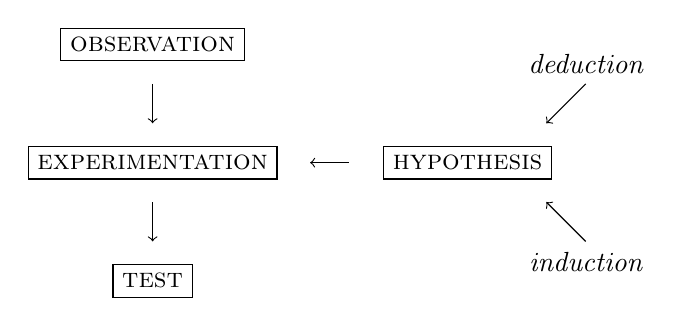
\begin{tikzpicture}
	\node[draw, align=center] at (0, 3.5) {\scshape observation};
		\draw[->] (0, 3) -- (0, 2.5);
	\node[draw, align=center] at (0, 2) {\scshape experimentation};
		\draw[->] (0, 1.5) -- (0, 1);
	\node[draw, align=center] at (0, 0.5) {\scshape test};
		\draw[<-] (2, 2) -- (2.5, 2);
			\node[draw, align=center] at (4, 2) {\scshape hypothesis};
				\draw[<-] (5, 2.5) -- (5.5, 3);
					\filldraw[black] (5.5, 3.5) node[anchor=north] {\itshape deduction};
				\draw[<-] (5, 1.5) -- (5.5, 1);
					\filldraw[black] (5.5, 0.5) node[anchor=south] {\itshape induction};
\end{tikzpicture}
\end{center}

\ex. Scientific hypotheses should be explicit enough that they make precise predictions that are testable. 
\a. Confirmations are never definitive proof of a theory.
\b. Unattended predicted observations may count towards falsification of a theory; however, apparent counterevidence may await a reanalysis.

\subsection{Pseudo-linguistics}

\ex. Language is a topic of endless fascination. As a consequence, any people seek to fascinate without bothering to find out if what they are saying about language is scientifically valid.
\a.The author is not engaged with the community of linguistics scholars.
\b. She conflates central concepts that are actually different. 
\c. She fails to engage with complex linguistic data.

\ex. Some examples:
\a. Australian speech patterns determined by drunk forefathers.
\b. Language change is predictable from humidity, altitude, etc.

\ex. Bigger, more dangerous problem: depiction of science in the media.


\subsubsection{Activity 4: Talk shop}

{\itshape Read each of the following statements and discuss them. What is your sentiment about them? Remember that there is no correct answer.}

\begin{enumerate}
\item The Sapir-Whorf hypothesis states that language and environment in which it is spoken are tightly connected, in such a way that they influence each other. There are two possible interpretations of such statement. A weak view argues that language has an effect on how we interpret the world; a stronger view holds that language defines and constrains our thoughts. 
	
	\begin{enumerate}
		\item[$\rightarrow$] Languages where gender agreement is marked, may reflect socio-political suprema\-cy of a gender class (e.g., men) over the other one (e.g., women).
	\end{enumerate}

\item Some dialects are inferior to others.
\item Esperanto is a constructed international auxiliary language ({\itshape auxlang}) invented in the late 1800s, with the aim of creating an easy-to-learn and politically neutral language that would transcend nationality and foster international cooperation.
\end{enumerate}

\section{Recap}

\ex. Until 1950s, language acquisition has been traditionally considered to an ability merely resulting from the mere behavioral response to a specific external stimulus. Noam Chomsky argued against such assumption and pointed out:
\a. child performance typically reaches its peak at age of 5, without active teaching being really effective ({\itshape \bfseries tacit knowledge}) and without a transparent input to refer to ({\itshape \bfseries poverty of stimulus});
\b. learning by memorization is empirically impossible, because we would need an incredible amount of memory to store all possible linguistic structures ({\itshape \bfseries open-ended creativity}).
\c. therefore, we must have an innate, universal set of rules for organizing language --- {\itshape Universal Grammar (UG)}.

\ex. Human language complexity is mainly due to three cognitive abilities: {\itshape \bfseries displaced reference, discreteness, recursion}.

\ex. As such, linguists are not interested in imposing rules, rather in describing and explaining structures {\itshape unconsciously} used by speakers; the term ``unconsciously'' refers to the fact that speakers do not explicitly know why, but they do know possible and impossible structures in a given language ({\itshape grammaticality}).

\ex. People interested in language should be wary of {\itshape pseudo-linguistics}. Linguistics, as all other sciences, must be pursued rigorously, in compliance with the Galilean scientific method.

\section{Selected references}

\begin{enumerate}
	\item Chomsky, N. (1959). A Review of B.F. Skinner's Verbal behavior. {\itshape Language}, 35(1), 26-58.
	\item Halle, M. (1973). Prolegomena to a Theory of Word Formation. {\itshape Linguistic Inquiry}, 4(1), 3-16.
	\item Skinner, B. F. (1957). {\itshape Verbal behavior}. Copley Publishing Group.
\end{enumerate}

\end{document}  